\addcontentsline{toc}{section}{Appendix} % Remove this if you don't want the appendix included in the table of contents.
\appendix

\section{MATLAB Code}\label{sec:matlab}
This section documents our MATLAB code.

\subsection{problem\_2.m}
\lstinputlisting[language=Matlab,caption={Problem 2 code},label=lst:problem_2]{../problem_2.m}
\subsection{compute\_lq.m}
\lstinputlisting[language=Matlab,caption={Script for computing the LQ k gain},label=lst:compute_lq]{../compute_lq.m}

\subsection{problem\_3.m}
\lstinputlisting[language=Matlab,caption={Problem 3 code},label=lst:problem_3]{../problem_3.m}
\subsection{problem\_4.m}
\lstinputlisting[language=Matlab,caption={Problem 4 code},label=lst:problem_4]{../problem_4.m}
\subsection{nonlcon.m}
\lstinputlisting[language=Matlab,caption={Nonlinear constraint function},label=lst:nonlcon]{../nonlcon.m}
\subsection{compute\_lq4.m}
\lstinputlisting[language=Matlab,caption={Compute LQ for the fourth problem},label=lst:compute_lq4]{../compute_lq4.m}

\subsection{plot2s3.m}
\lstinputlisting[language=Matlab,caption={Plot the test run for case 10.2},label=lst:plot2s3]{../plot2s3.m}
\subsection{plot3s3.m}
\lstinputlisting[language=Matlab,caption={Plot the test run for case 10.3},label=lst:plot3s3]{../plot3s3.m}
\subsection{plot4s3.m}
\lstinputlisting[language=Matlab,caption={Plot the test run for case 10.4},label=lst:plot4s3]{../plot4s3.m}

\section{Simulink Diagrams}\label{sec:simulink}
This section contains Simulink diagrams.

\subsection{No Feedback}
\begin{figure}[H]
	\centering
		\includegraphics[scale=0.3]{figures/{2-simulinksim_helicopter}.eps}
	\caption{The simulink model used for optimal open loop control.}
\label{fig:2-simulink}
\end{figure}

\subsection{Feedback (LQ)}
\begin{figure}[H]
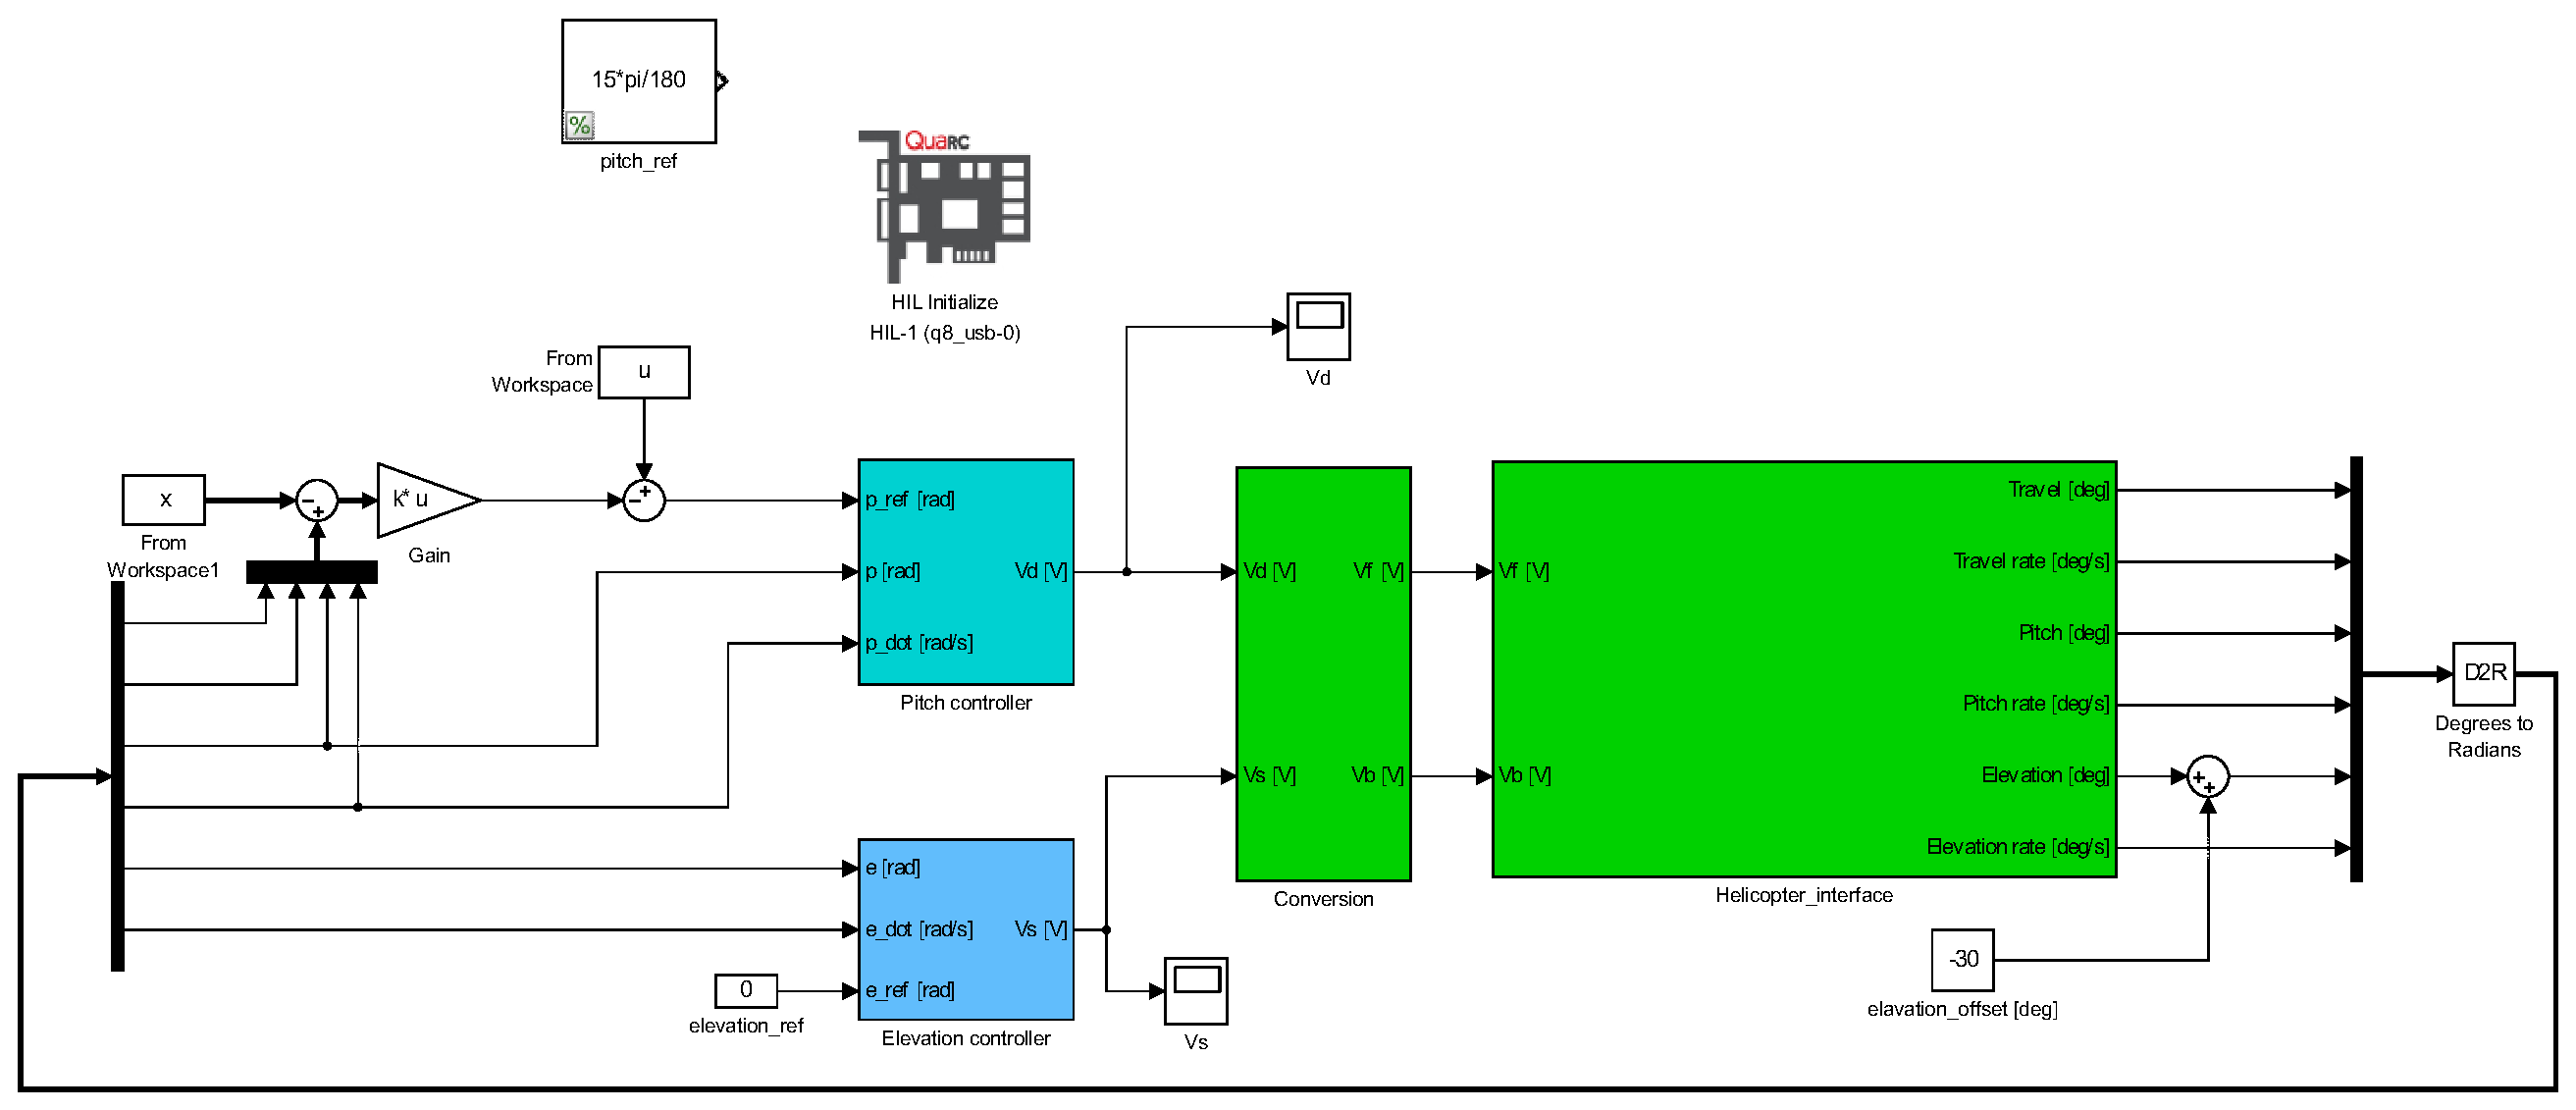
\includegraphics[scale=0.3]{figures/3-simulinksim_helicopter.eps}
\caption{Feedback system for the helicopter with static elevation control}
\label{fig:feedback-3}
\end{figure}

\subsection{Pitch and Elevation Control}
\begin{figure}[H]
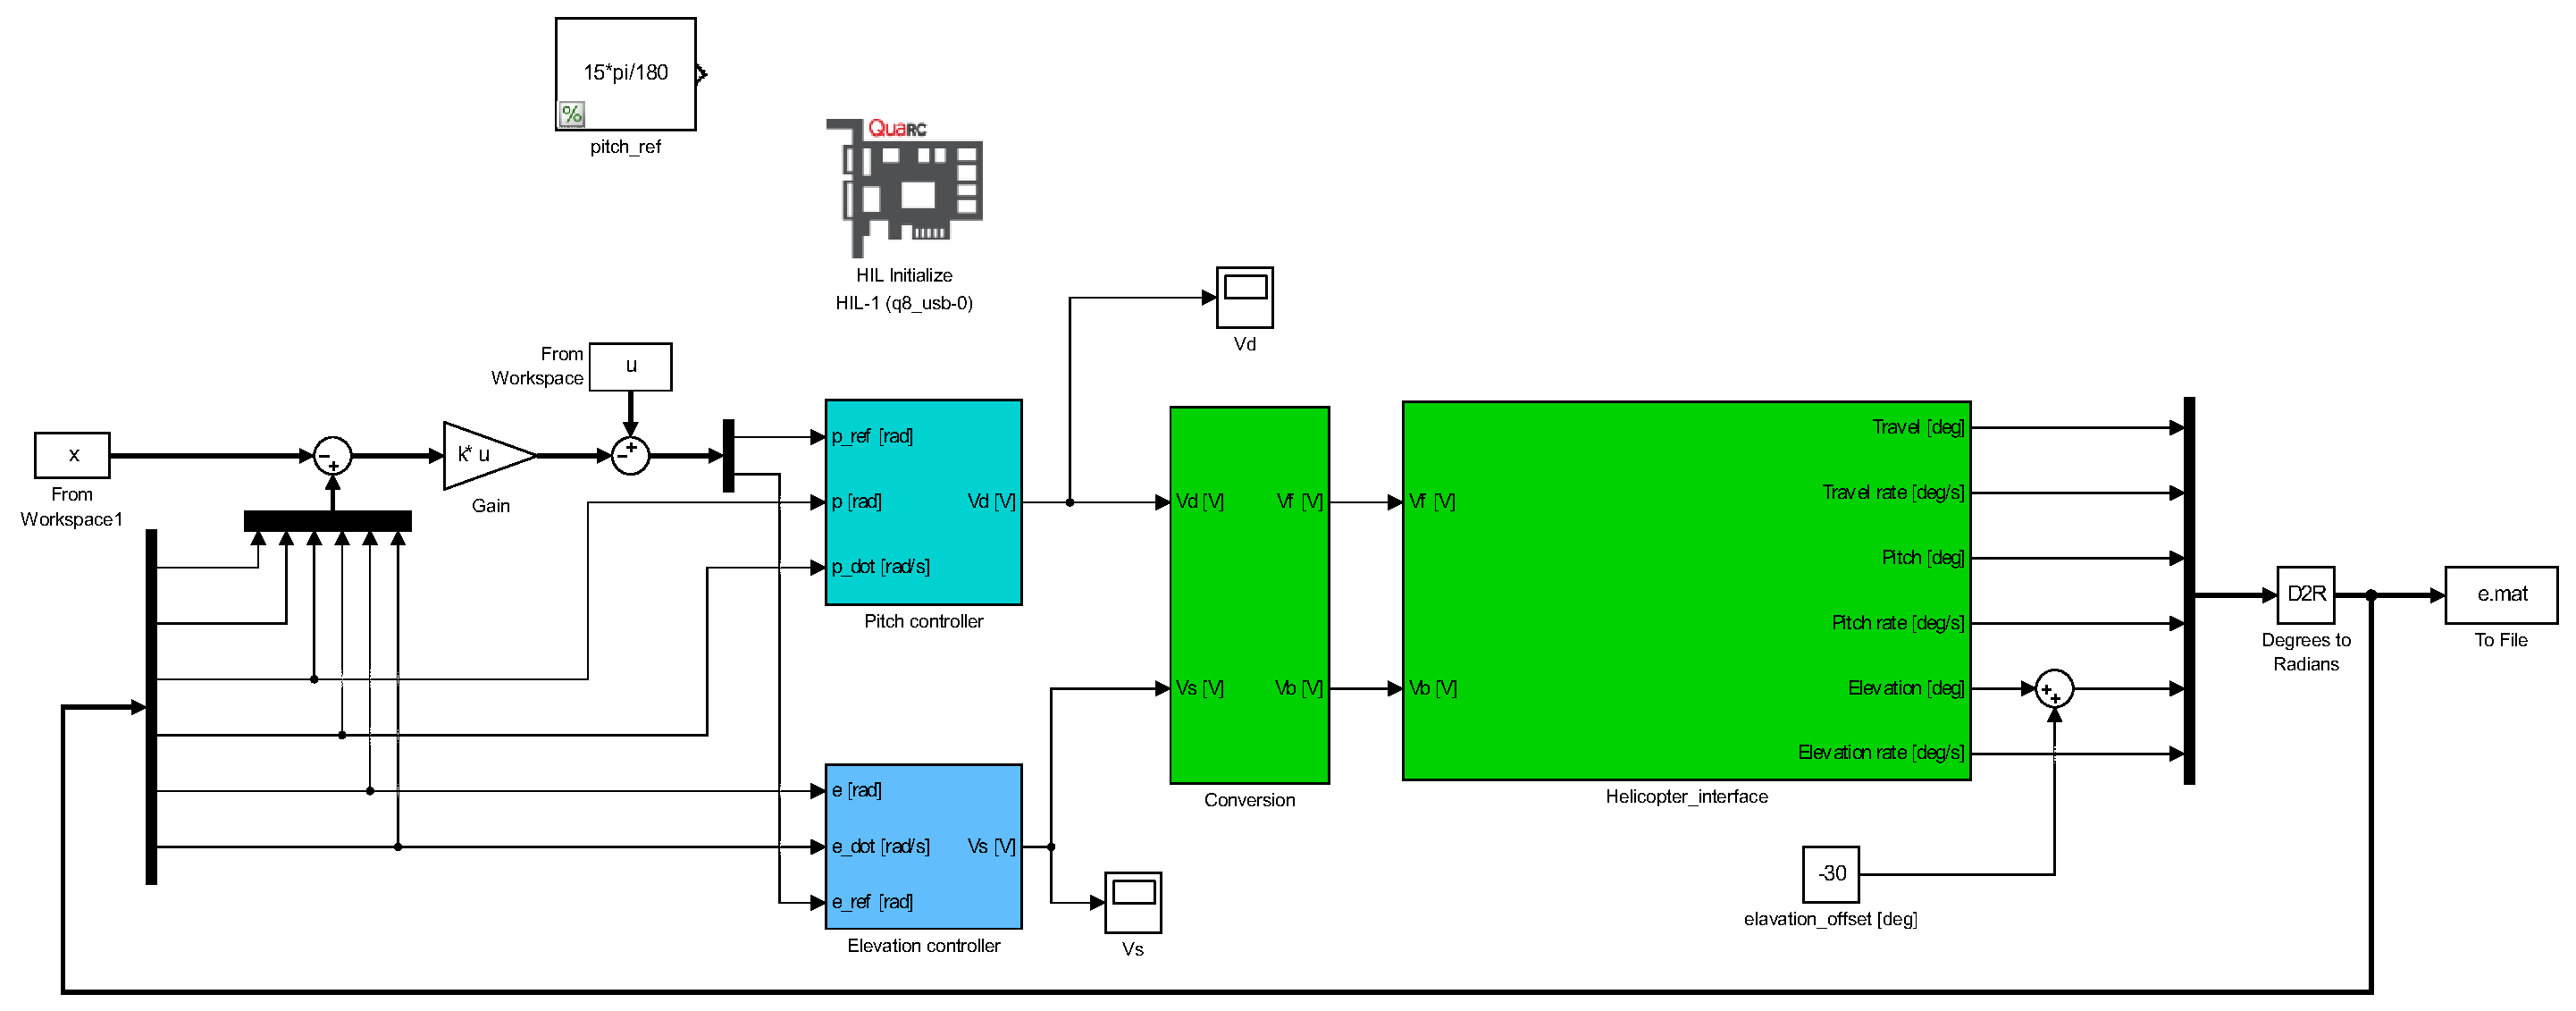
\includegraphics[scale=0.3]{{figures/4-simulinksim_helicopter}.eps}
\caption{Feedback system for the helicopter (N=40), for the non-feedback case the constant gain is zerod.}
\label{fig:feedback-4}
\end{figure}

\section{Lab exercises}\label{sec:ex}

\includepdf[pages={-}]{LabExercise.pdf}

